\documentclass[column,brazilian,12pt,a4paper,final]{article}
\usepackage[brazil]{babel}
\usepackage{nonfloat}
\usepackage[utf8]{inputenc}
\usepackage{multicol}
\usepackage{hyperref}
\usepackage[pdftex]{color,graphicx}
\usepackage{geometry}
\usepackage{amsmath}
 \geometry{
 a4paper,
 total={170mm,257mm},
 left=20mm,
 top=20mm,
 }
 \usepackage{ragged2e}
\usepackage{fancyhdr}
\usepackage{caption}[=v1]
\usepackage{xcolor}
\pagestyle{plain}
\fancyhead{}
\lhead{
\includegraphics[width=1.5cm]{logoufrgs}}
\rhead{
\includegraphics[width=0.8cm]{logoif}}
\fancyfoot{}
\fancyhead[C]{\footnotesize Física Experimental III $\bullet$ 2025/1}
\fancyfoot[RO,LE]{\thepage}
\usepackage{float}
\usepackage{setspace}


\title{Estudo do Campo Elétrico a Partir de Equipotenciais }
\author{Autores: \\ Lucas Assis Paulino da Silva - 590174 \\Lucas Bertazo de Deus Félix - 587064
 \\ Pedro Henrique Reis de Oliveira - 590908 \\ IF-UFRGS}
\date{Abril 2025}

\begin{document}
\maketitle
\thispagestyle{fancy}

\section*{Resumo}
\paragraph{}

No que diz respeito ao estudo da eletrostática, este relatório possui como objetivo analisar dados coletados em uma montagem experimental que permitiram a visualização das equipotenciais entre dois extremos de um dipolo elétrico. Com tais dados pudemos, então, processar a partir de métodos computacionais os valores obtidos em cada ponto equipotencial e derivar o campo elétrico dos mesmos. Tal procedimento possibilitou a visualização gráfica do pressuposto teórico de campo elétrico reafirmando a geometria esperada para este cenário. Devemos ressaltar o aspecto da incerteza inerente à como as medidas foram tomadas; a ponteira utilizada para medir o potencial em cada ponto foi operada manualmente e o papel milimetrado de referencia possui incerteza visual de ±0,05cm além da propagação de incertezas no processo derivativo. Considerando tal aspecto, pudemos calcular ainda o valor do campo nos pontos (5;0), (0;0), (-5;0) e (5;5) como sendo (+0,3183;-0,0096) e módulo igual a 0,3183, (+0,2319;0,0000) e módulo igual a 0,2319, (+0,3620;-0,0277) e módulo 0,3631 e (0,2311;0,0753) e módulo igual a 0,2431 respectivamente. 

\section{Introdução}
\paragraph{}

Tratando do estudo da eletrostática, as linhas de campo imaginárias têm papel fundamental no processo de abstração e interpretação dos fenômenos físicos inerentes ao comportamento das cargas em nosso universo. Tal princípio foi o motivador para a realização do experimento aqui relatado. Construindo-se uma estrutura que nos permitisse medir coordenadas de pontos equipotenciais, a visualização gráfica dos mesmos, por si só, nos ajudam a compreender a geometria presente nos fenômenos elétricos que nos rodeiam. Entretanto, explorando a base teórica física e matemática construída até o momento, podemos ir ainda além, relacionando as medidas de diferença de potencial com a definição do campo elétrico e seu aspecto vetorial. Dessa forma, esperamos que linhas de campo perpendiculares àquelas das equipotenciais se formem ao construirmos seus respectivos gráficos e façamos o processamento de dados necessário.  

\section{Embasamento Teórico}
\paragraph{}
Posto um sistema elétrico dipolar, nos baseamos nas linhas de campo para idealizar e definir o comportamento vetorial do campo elétrico gerado por ele. Nossa teoria afirma que as linhas de campo "saem" da carga positiva do sistema e se conectam com as linhas de campo do polo negativo que as recebem. Nosso intuito em estudar experimentalmente o sistema supracitado é de visualizar essas linhas e montar gráficos, não somente teóricos, das linhas de campo do sistema. Podemos, ainda, chamar a diferença de potencial em cada ponto de DDP, ou também de voltagem[V]. Esse termo que utilizaremos daqui a diante. Como citado anteriormente, a relação existente entre as voltagens medidas e o vetor campo elétrico é o princípio da nossa análise. Essa relação se mostra da seguinte maneira:

\subsection{Campo Elétrico e Voltagem:}

\begin{equation}
    \Vec{E} = -(\frac{\partial V}{\partial x}\vec{i} + \frac{\partial V}{\partial y}\vec{j} + \frac{\partial V}{\partial z}\vec{k})
\end{equation}

A igualdade acima expressa a relação existente entre o vetor campo elétrico e a voltagem como sendo o negativo do vetor gradiente formado pelas derivadas parciais da função escalar de $V$ em cada ponto. O que reafirma a ideia do vetor campo elétrico ser perpendicular as linhas equipotenciais do sistema. 

\section{Material Utilizado}
\begin{itemize}
    \item Minipa® ET-2075B(Multímetro)
    \item Cilindro condutor(3,5cm de diâmetro)
    \item Placas metálicas(5cm de largura)
    \item Fonte Elétrica - IF UFRGS
    \item Suportes Condutores 
    \item Eletrodos
    \item Presilhas
    \item Papel milimetrado
    \item "Bacia" retangular 

\end{itemize}
\section{Procedimentos e Montagem}
\paragraph{}
No  que concerne o método experimental utilizado, estruturamos sobre o papel milimetrado uma "bacia" de vidro fina sobre a qual foram conectados duas terminações de um circuito elétrico. Estes que saíam de uma fonte de alimentação que gerava um DDP total de aproximadamente 10V. A montagem se encontra na ilustração a seguir(Figura 1):
\singlespacing


    \centering
    \begin{minipage}{0.45\textwidth}
        \centering
        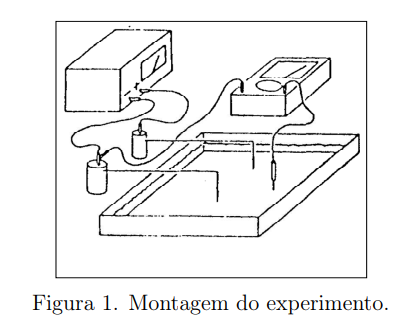
\includegraphics[width=\linewidth]{MECE.png}
      
        \label{fig:imagem1}
    \end{minipage}
    \hfill
    \begin{minipage}{0.45\textwidth}
        \centering
        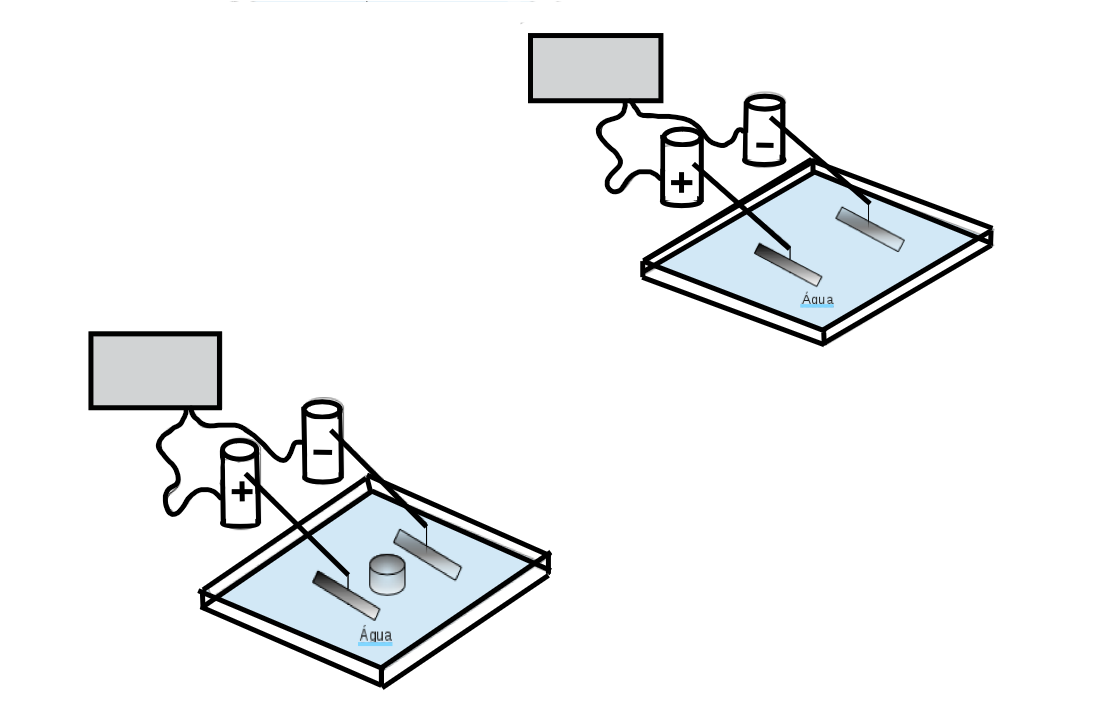
\includegraphics[width=\linewidth]{MECEII.png}
        \caption{Figura 2. Montagem do Experimento II}
        \label{fig:imagem2}
    \end{minipage}


\justifying 

\paragraph{}
Definida nossa montagem experimental, a coleta de dados se deu por meio de um multímetro, o qual foi operado manualmente, o que gerou incerteza de medida inerente ao método, conectado ao sistema. Cada medida consistia-se das coordenadas do ponto e a voltagem medida naquele ponto. Dessa forma, possuiríamos os dados necessários para a construção de um gráfico de equipotenciais e posterior processamento de dados para determinação do campo elétrico em cada situação estruturada. Devemos ressaltar também que, além da montagem expressa acima, também foram feitas medidas onde barras metálicas se encontravam lado a lado sobre cada polo, gerando um campo teoricamente linear uniforme, e por fim, um cilindro metálico adicionado no centro entre as duas barras(Figura 2).





\section{Dados Experimentais}
\subsection{Medidas Equipotenciais - I:}
\paragraph{}
Neste experimento em específico, todos os dados coletados foram claramente expressos nos gráficos que procederão a seguir. Dito isto, aqui constarão somente alguns exemplos tabelados dos dados coletados, contendo as coordenadas de cada ponto e a voltagem medida para a primeira configuração(montagem I):

\linespread{1}
\begin{table}[h!]
\centering
\vspace{0.5cm}
\begin{tabular}{c|c|c}
\hline
   X[cm]  &  Y[cm] & Volts[$V$]
   \\
   \hline
   0 & 0& 5\\
   0 & -10&5 \\
   0 & -5&5 \\
   0 & 5& 5\\
   0 & 10& 5\\
   7,5 & 0& 3,36\\
   8 & -1,4& 3,36\\
   9 & -2,6 & 3,35\\
   8 & 1,4& 3,37\\
   9 & 2,5& 3,37\\
   . & . & .\\
   .&.&.\\
   \hline
\end{tabular}
\linespread{1}
\end{table}
\justifying

\subsection{Gráficos Equipotenciais e de Campo Elétrico:}

    \centering
    \begin{minipage}{0.48\textwidth}
        \centering
        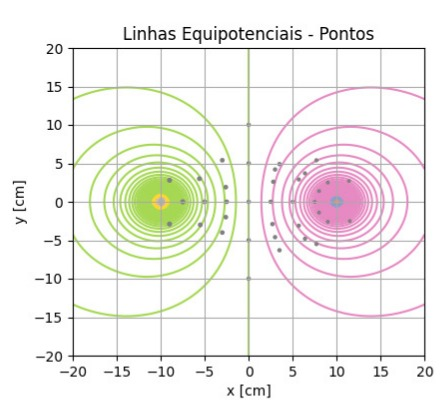
\includegraphics[width=\linewidth]{EP1.jpg}
        
        \label{fig:imagem1}
    \end{minipage} \hfill
    \begin{minipage}{0.48\textwidth}
        \centering
        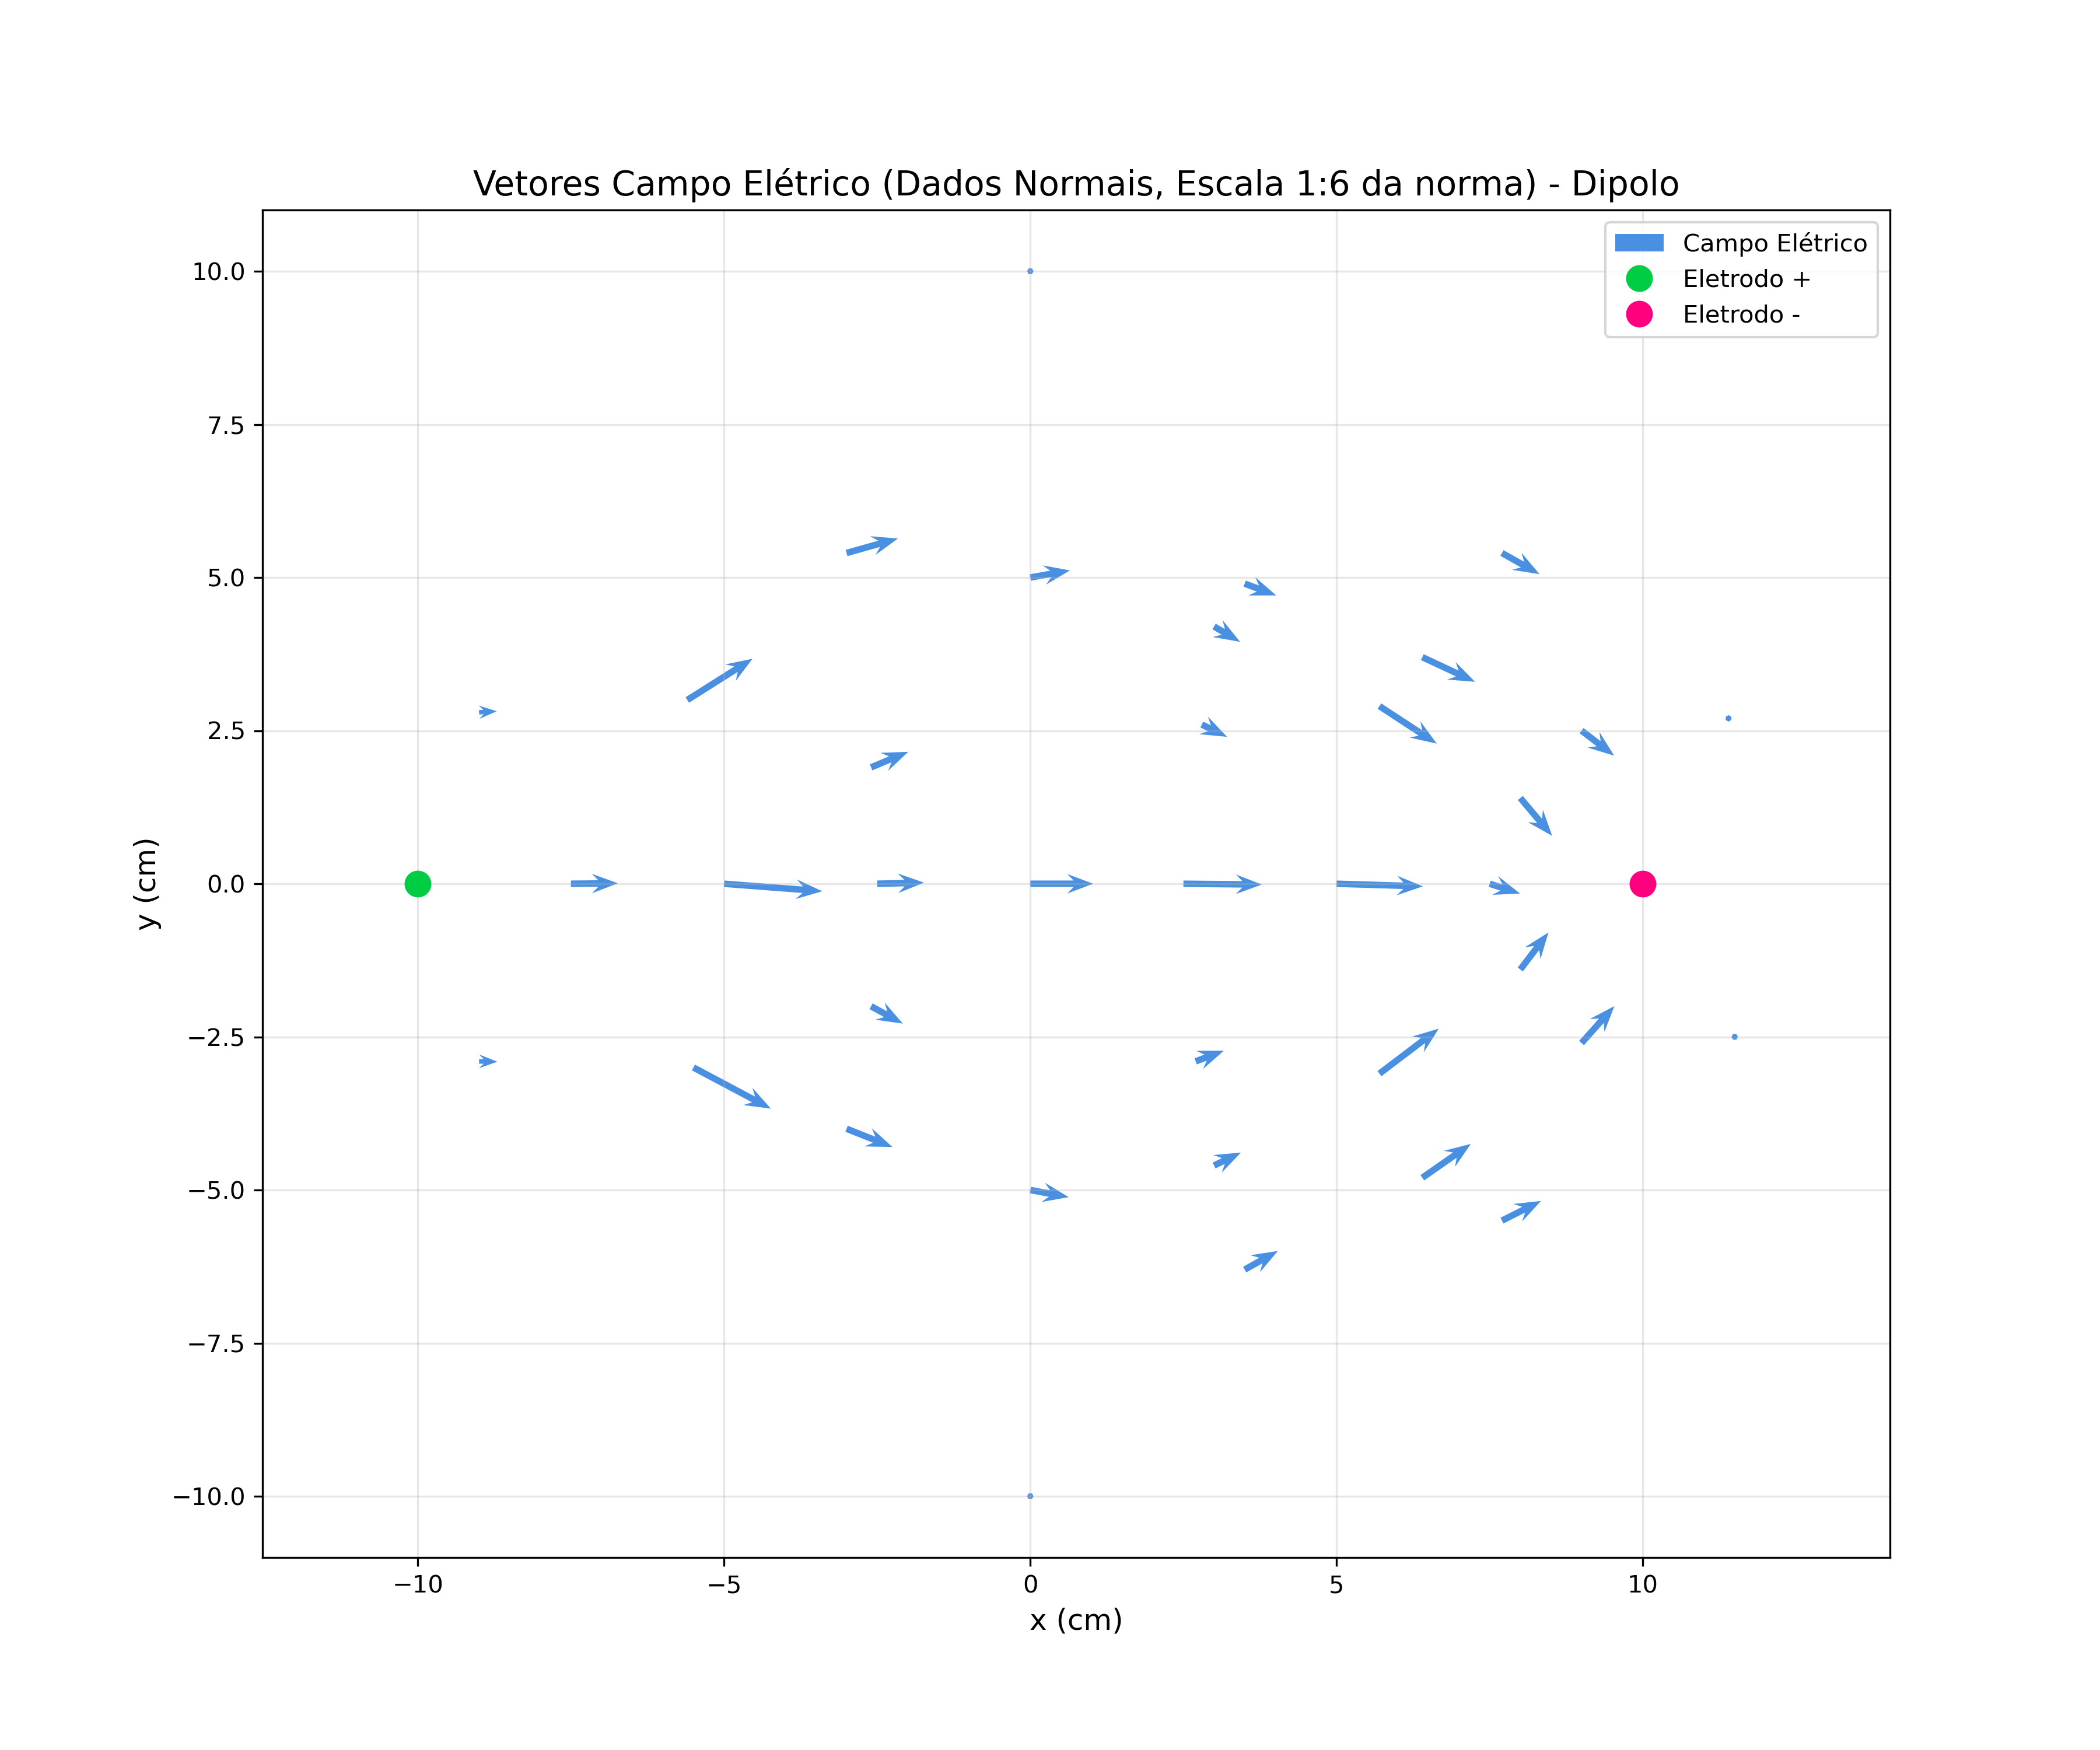
\includegraphics[width=\linewidth]{Campo DipoloN.png}
        \label{fig:imagem2}
    \end{minipage}
    
    \vskip 0.5cm % Space between rows
    
    % Second Row
    \begin{minipage}{0.48\textwidth}
        \centering
        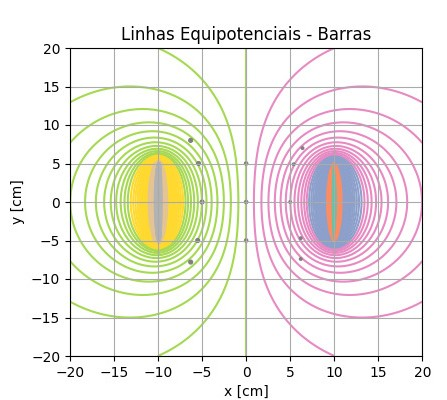
\includegraphics[width=\linewidth]{EP2.jpg}
        \label{fig:imagem3}
    \end{minipage} \hfill
    \begin{minipage}{0.48\textwidth}
        \centering
        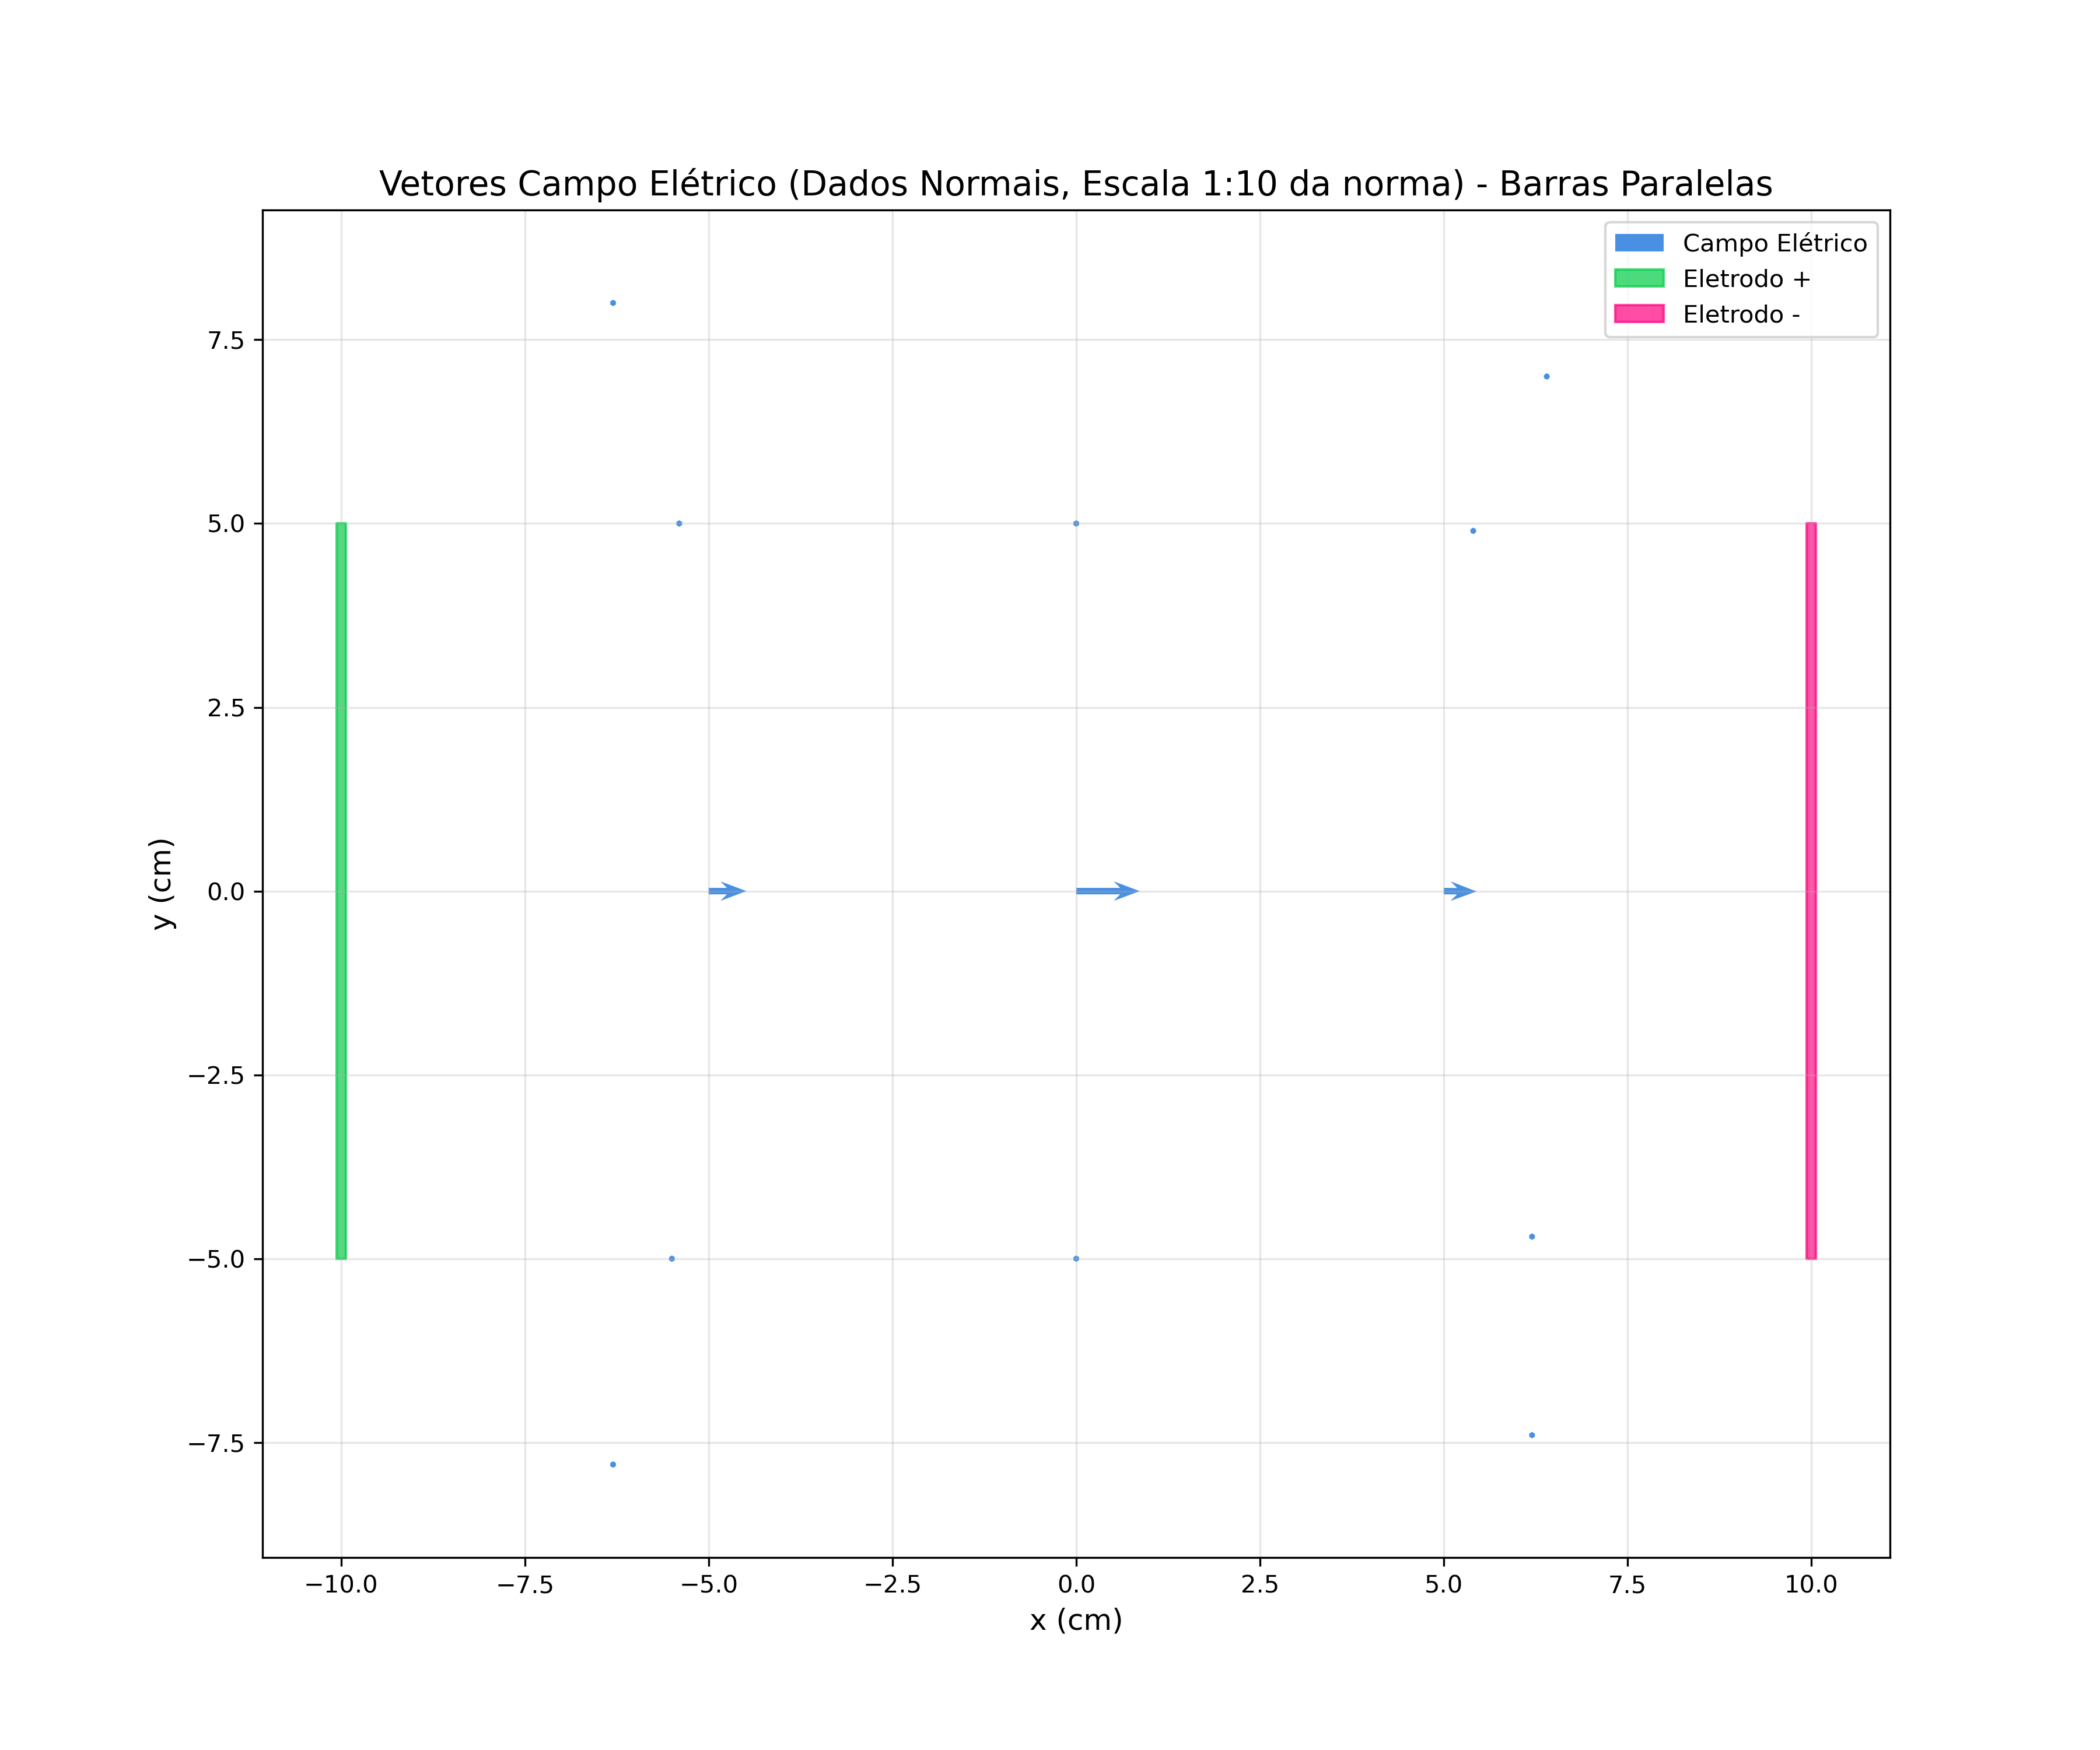
\includegraphics[width=\linewidth]{Campo PlacasN.png}
        \label{fig:imagem4}
    \end{minipage}
    
    \vskip 0.5cm % Space between rows
    
    % Third Row
    \begin{minipage}{0.48\textwidth}
        \centering
        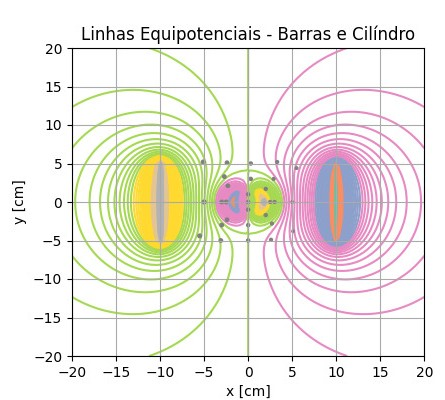
\includegraphics[width=\linewidth]{EP3.jpg}
        \label{fig:imagem5}
    \end{minipage} \hfill
    \begin{minipage}{0.48\textwidth}
        \centering
        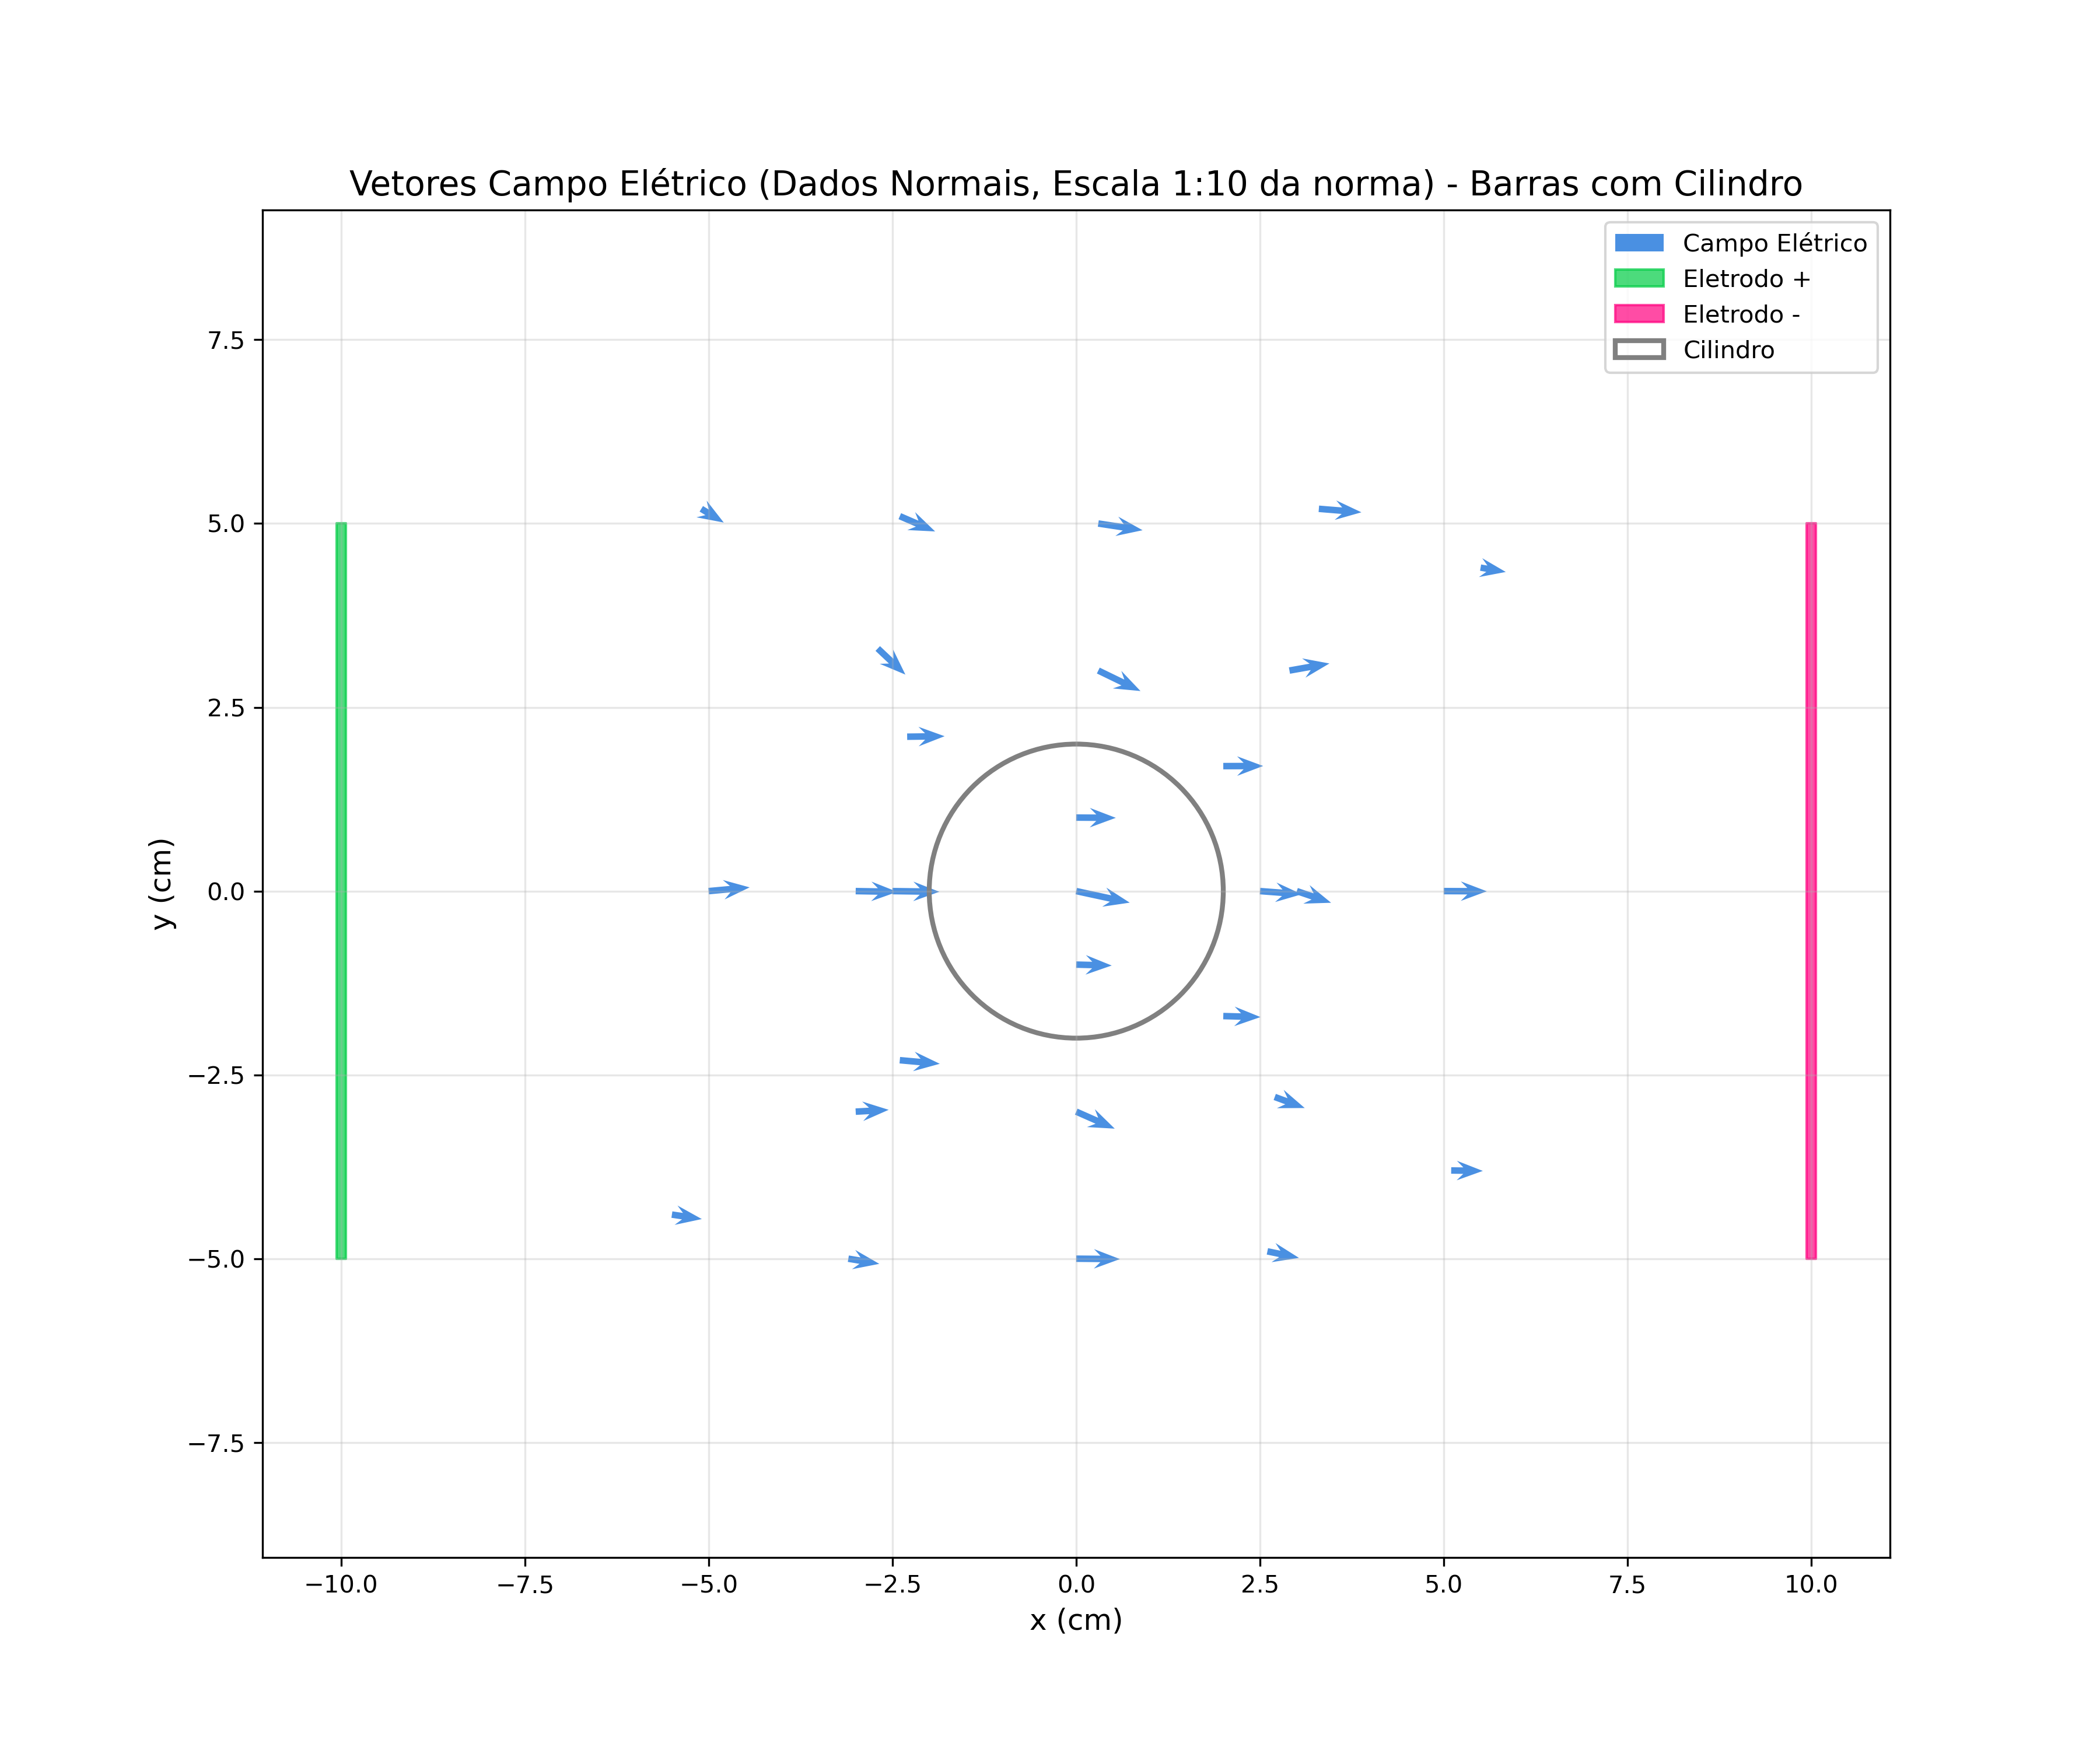
\includegraphics[width=\linewidth]{Campo CilindroN.png}
        \label{fig:imagem6}
    \end{minipage}


\justifying 

\subsection{Gráficos Interpolados de Campo Elétrico }
    \centering
    
    \centering
    \begin{minipage}{0.8\textwidth}
\begin{figure}
            \centering
            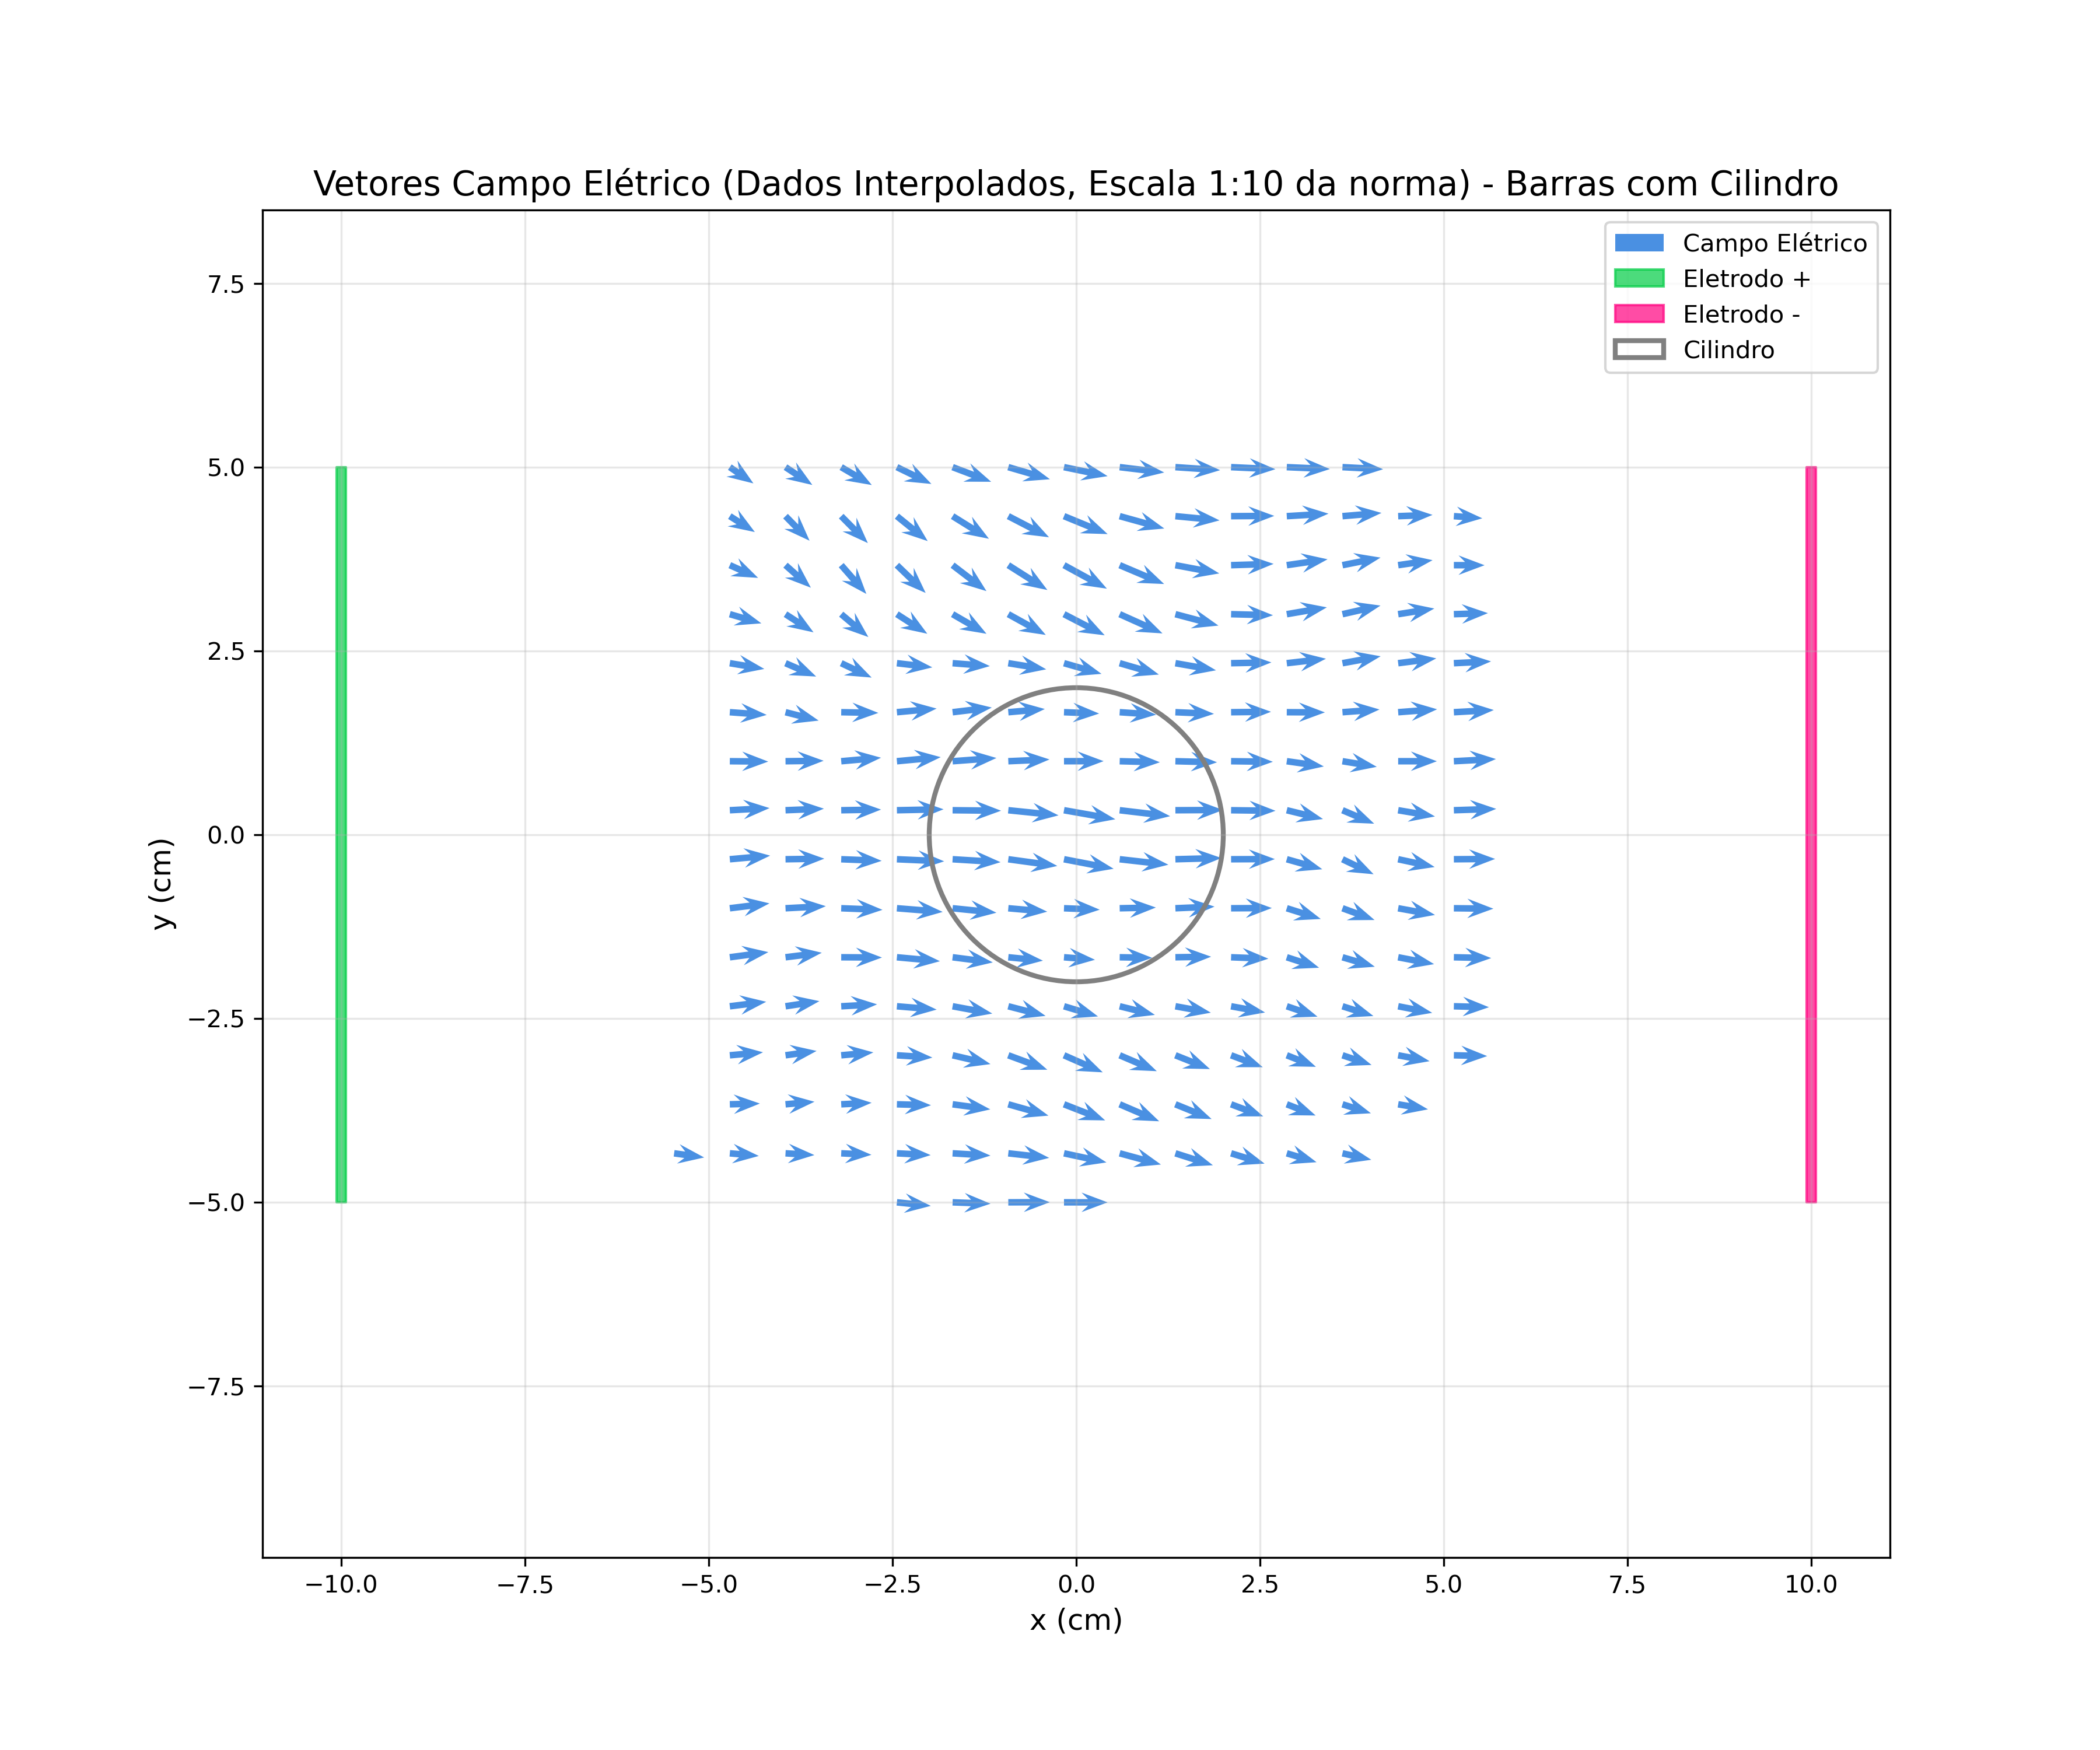
\includegraphics[width=0.5\linewidth]{Campo Cilindro.png}
            \caption{Enter Caption}
            \label{fig:enter-label}
        \end{figure}
                \centering
        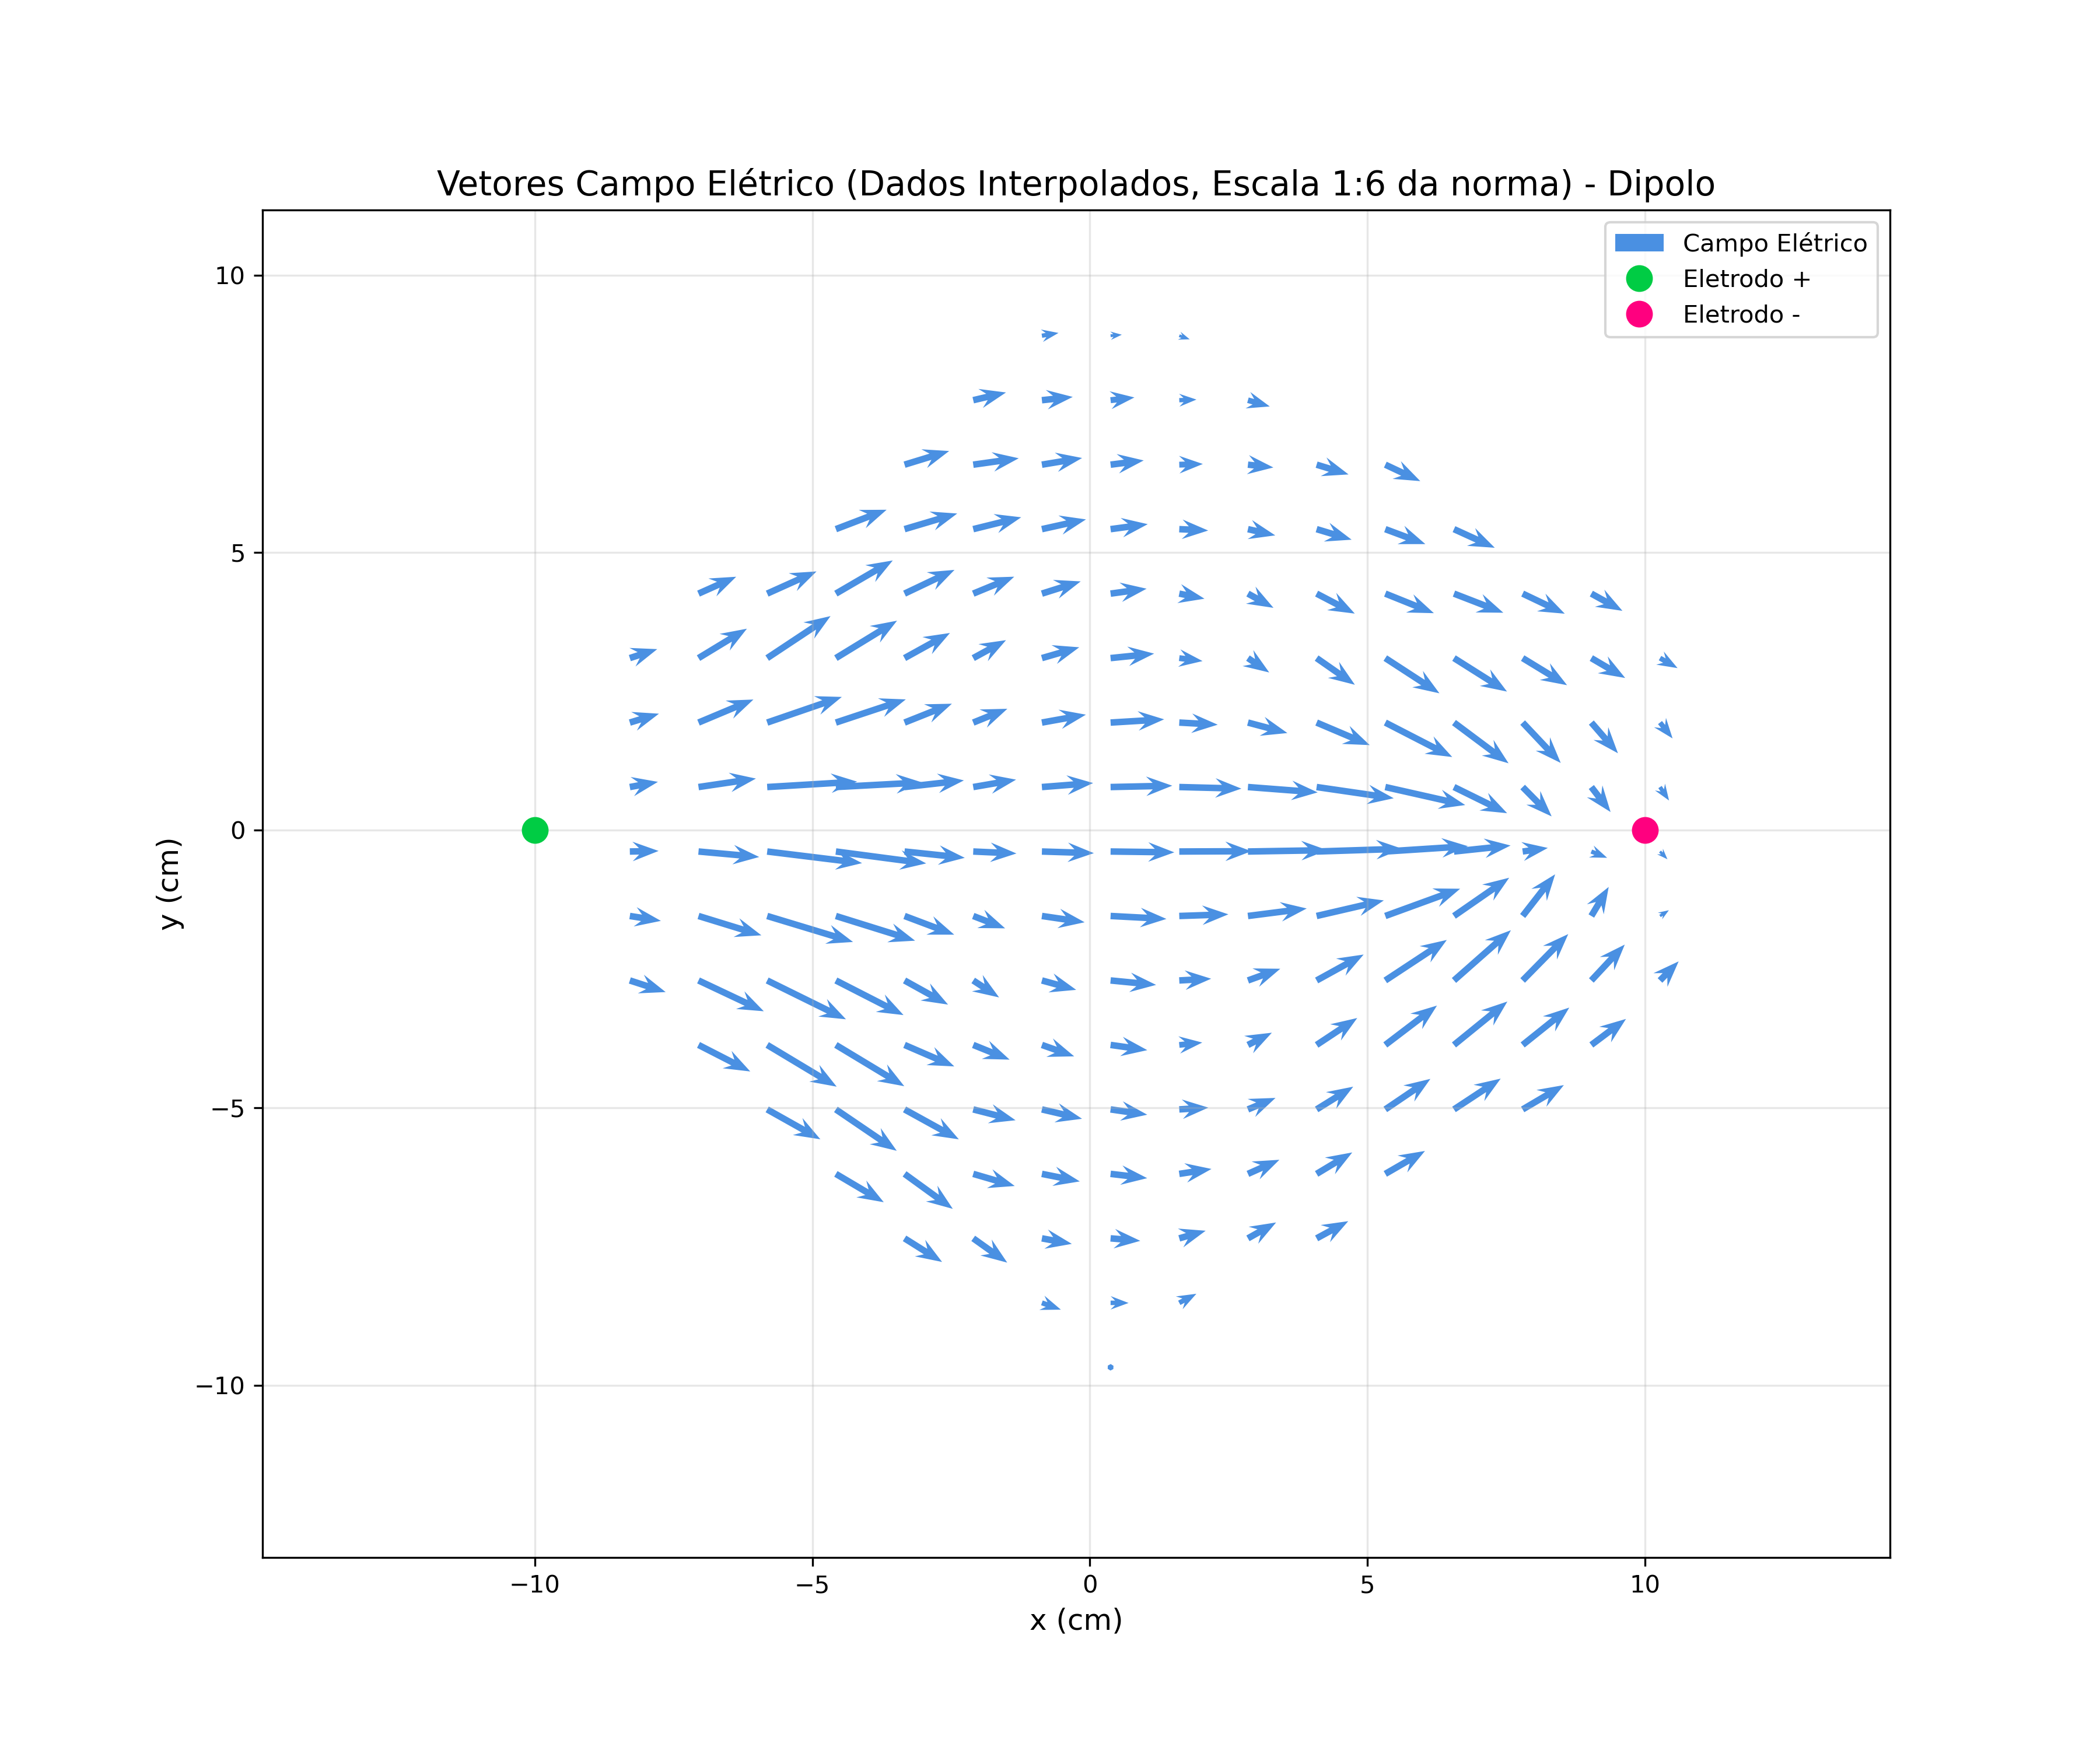
\includegraphics[width=\linewidth]{Campo Dipolo .png}
        \label{fig:imagem1}
    \end{minipage}
    \hfill
    \begin{minipage}{0.8\textwidth}
        \centering
        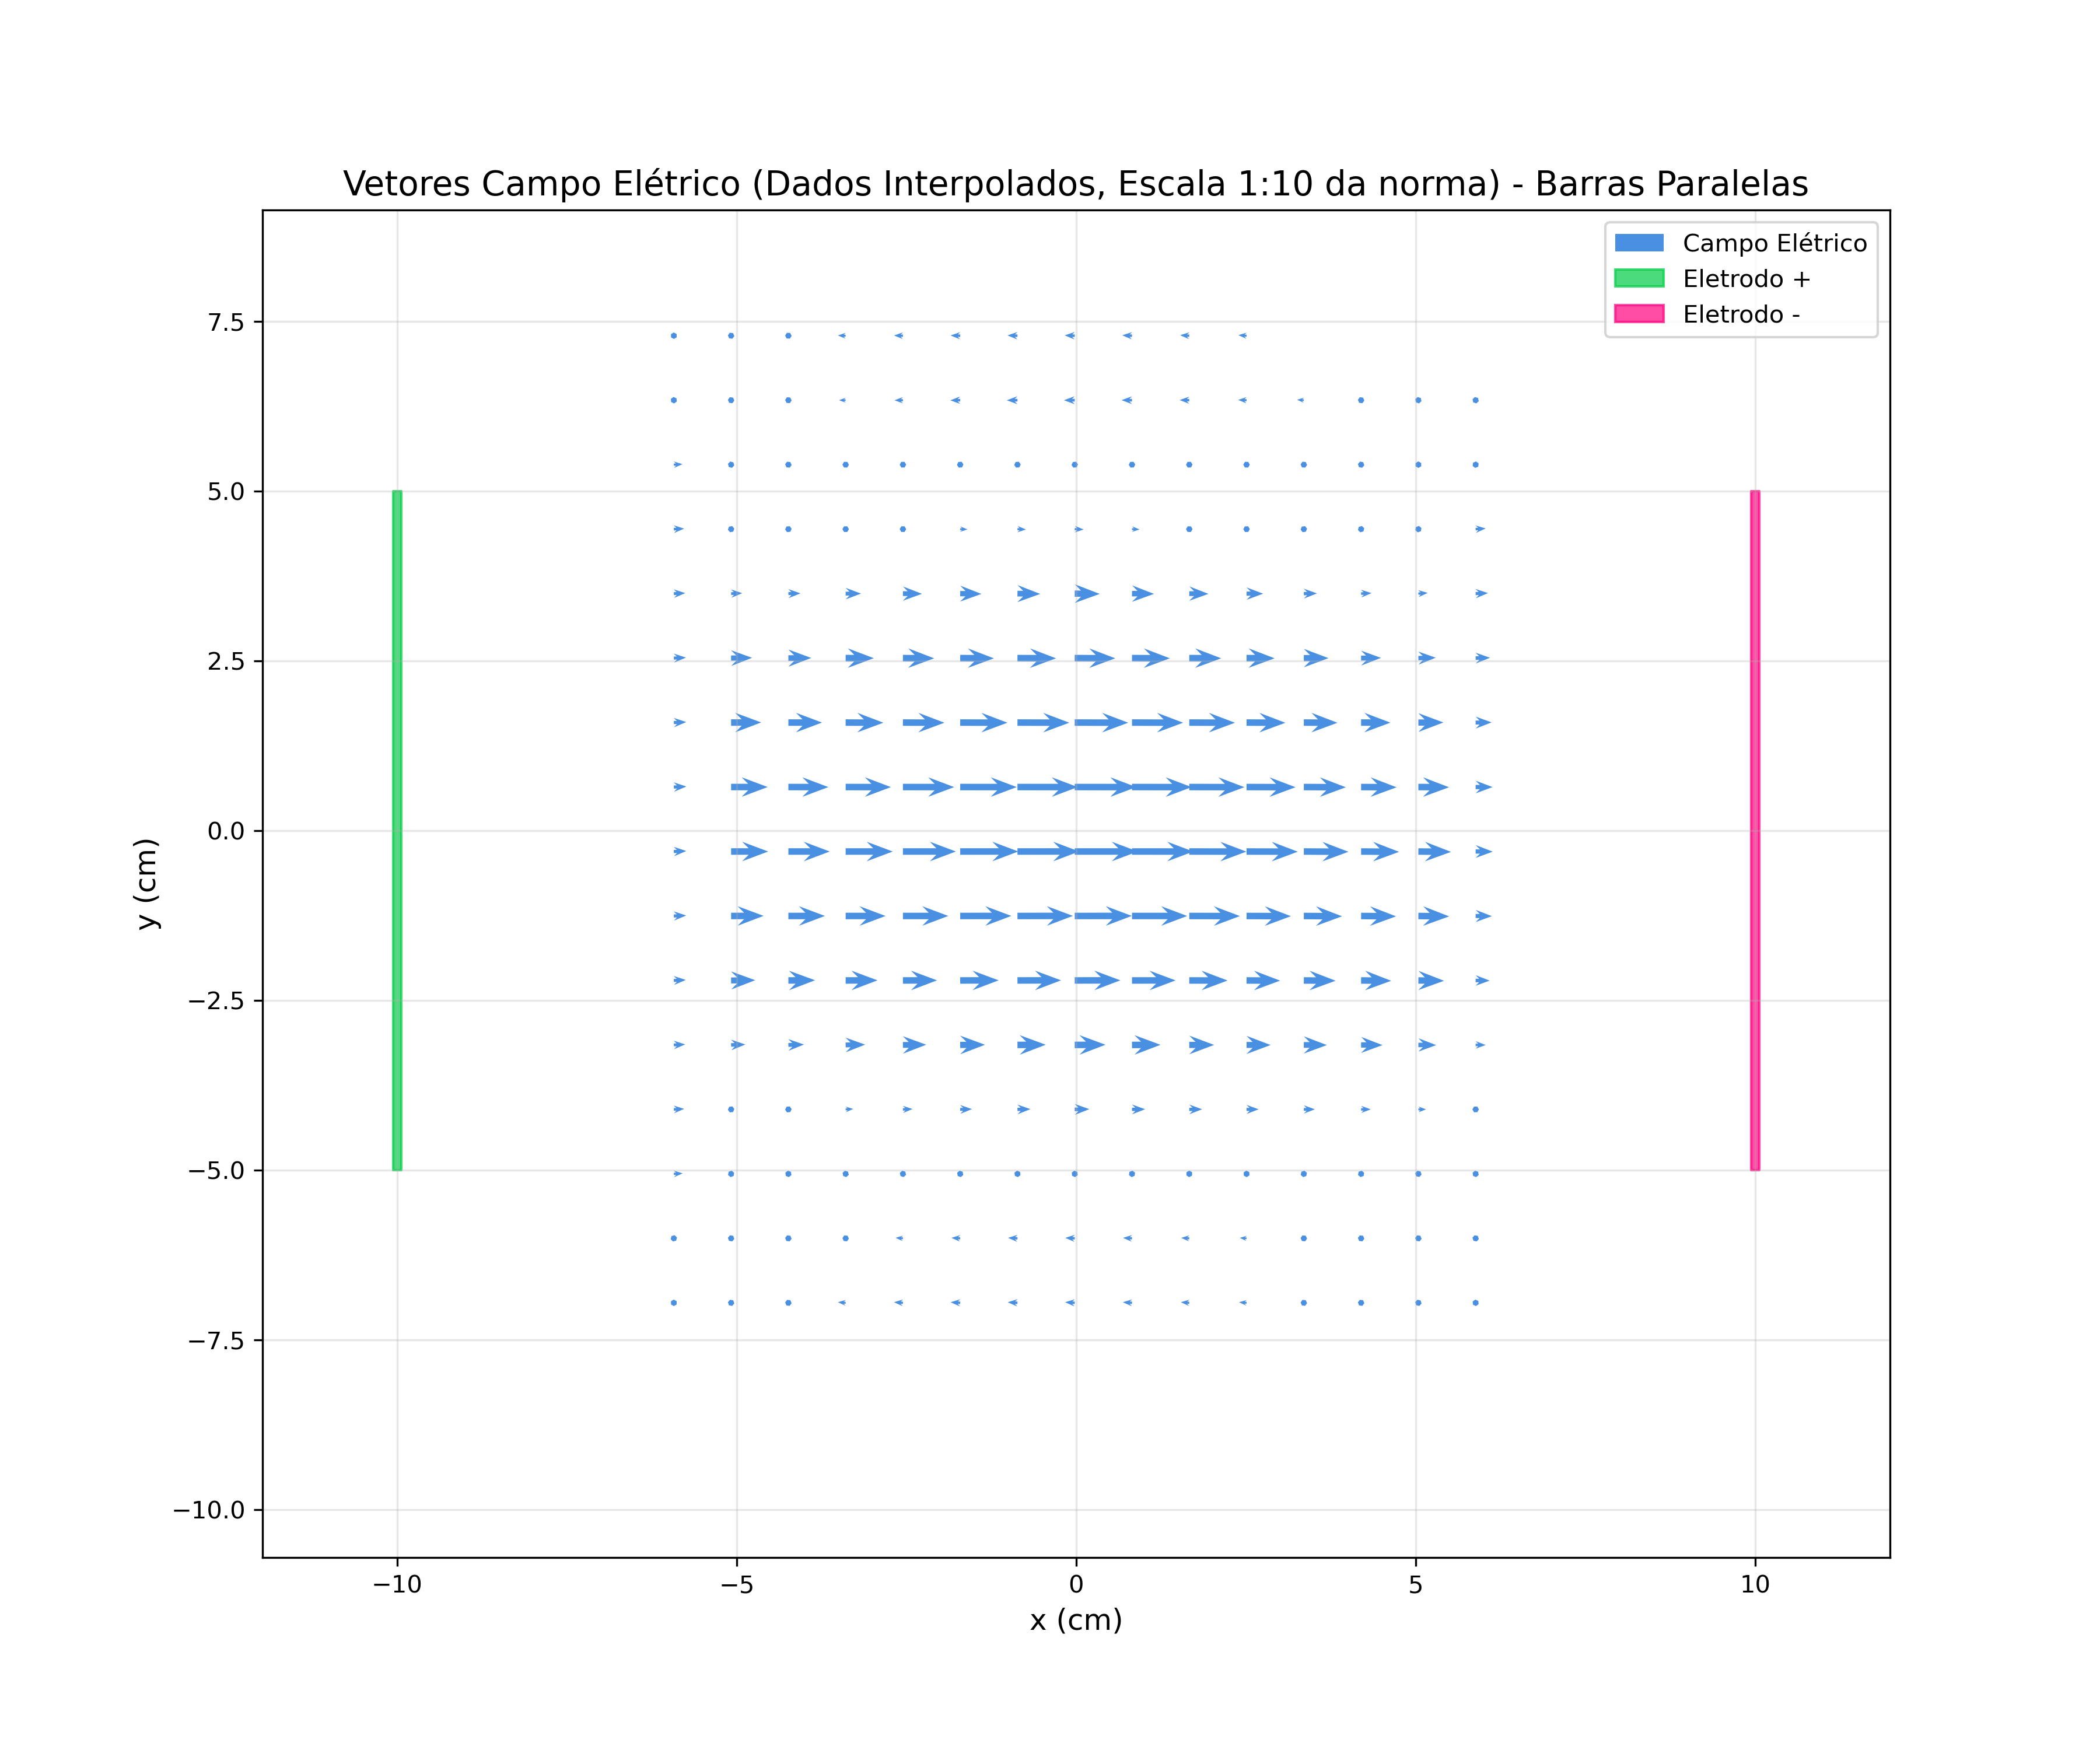
\includegraphics[width=\linewidth]{Campo Placas.png}
       
        \label{fig:imagem2}
    \end{minipage}
 \begin{minipage}{0.8\textwidth}
    \centering
    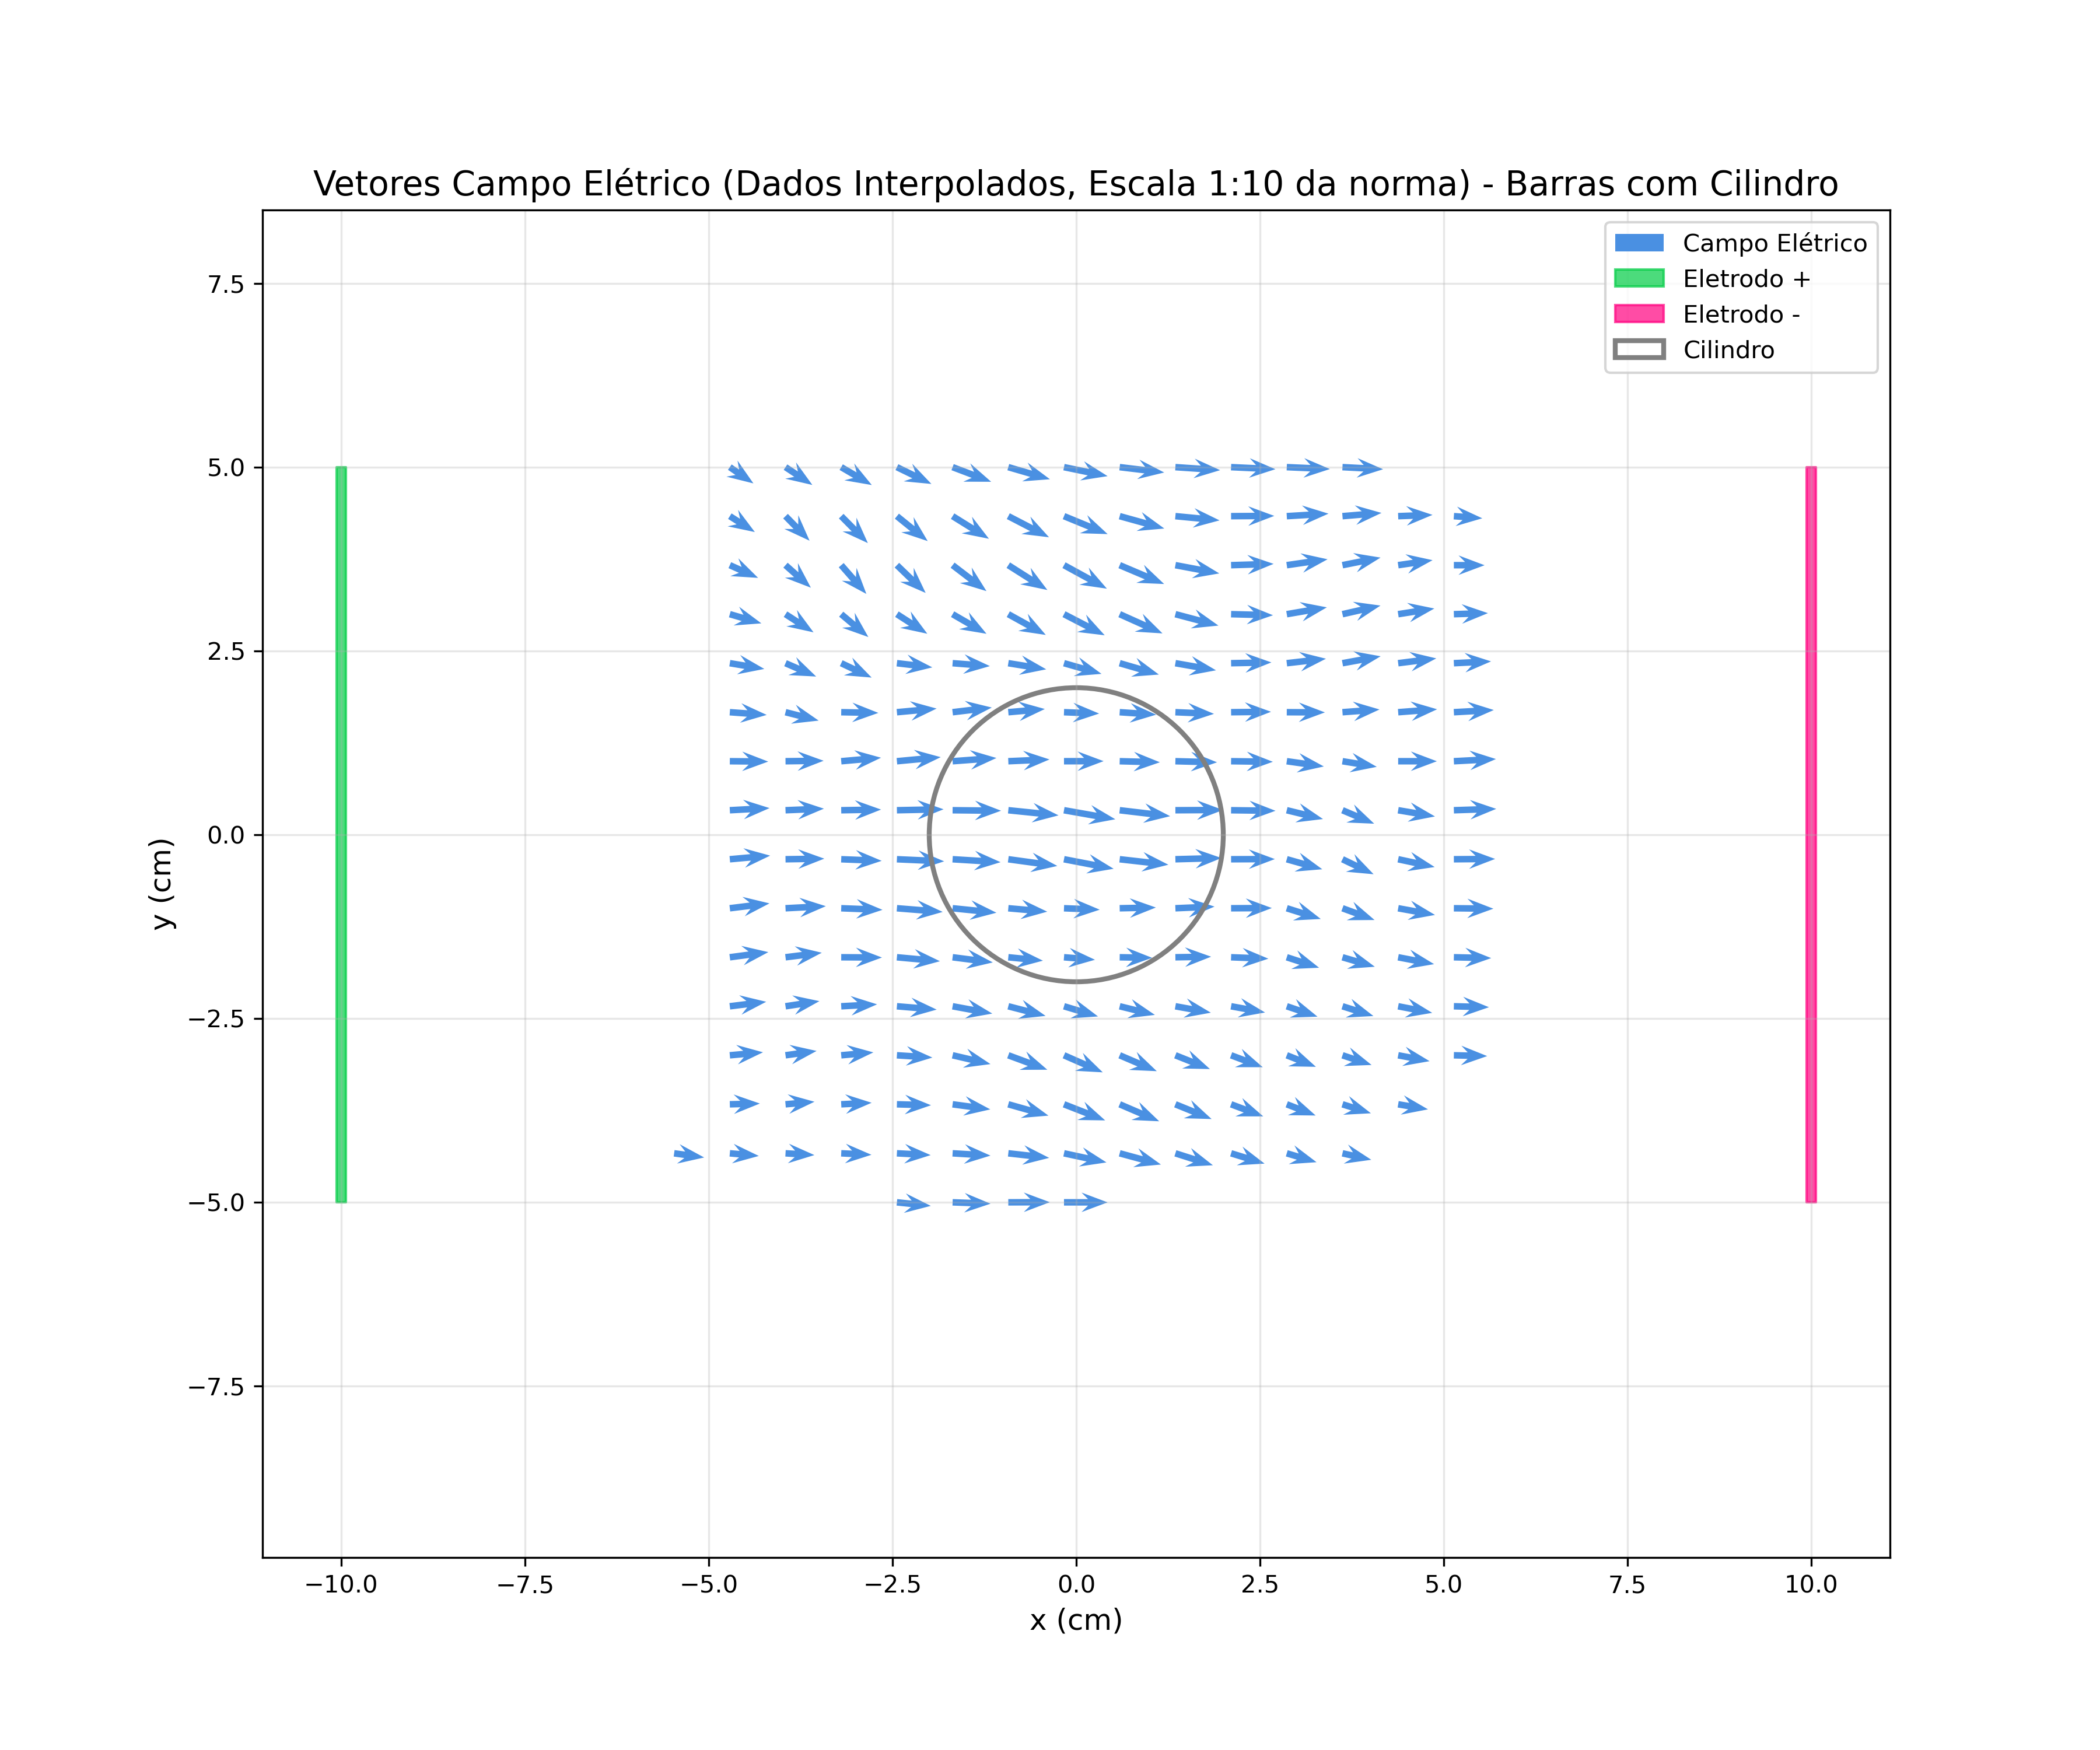
\includegraphics[width=\linewidth]{Campo Cilindro.png}
    \label{fig:enter-label}
\end{minipage}
    \centering






\justifying
\subsection{Gráfico do Potencial Sobre o Eixo X}
O gráfico a seguir corresponde à variação da voltagem medida rente ao eixo X do sistema constituído pelo dipolo isolado: o potencial diminui linearmente conforme nos afastamos do polo positivo. 
\begin{figure}[H]
    \centering
    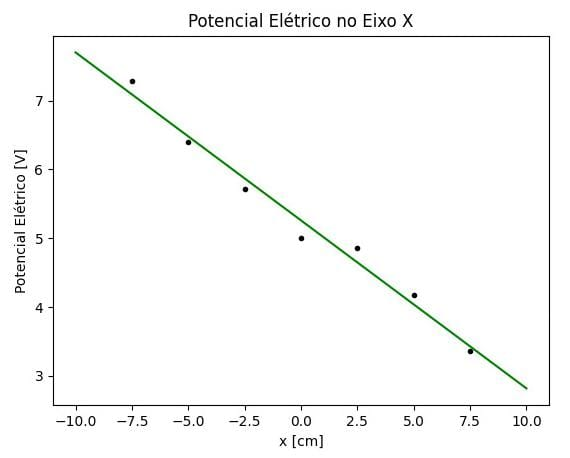
\includegraphics[width=0.5\linewidth]{DPx.jpg}
\end{figure}
O gráfico acima corresponde à primeira parte da questão 2 do trabalho presente no roteiro do experimento.  


\justifying
\section{Análise de Dados}
\paragraph{}
Trazendo à tona a premissa do experimento, os gráficos das equipotenciais e dos campos, produzidos a partir de um delicado trabalho computacional(Acesse o tratamento computacional de dados completo em: \url{https://github.com/sunbaee/Eletrostatics} e \url{https://github.com/pedro-hro/Relatorio_1-ExperimentalIII/tree/master}), decerto reproduziram aquilo idealizado ante à teoria em questão, entretanto, cada configuração experimental com suas peculiaridades. Traçando como linhas os pontos coletados sob certa restrição de potencial similar, a configuração 1 do experimento torna nítido o comportamento de projeções circulares de equipotenciais ao redor dos centros de carga, encontrando um ponto médio perpendicular ao eixo do dipolo. \footnote{Resposta à questão 6ai do trabalho no roteiro}Além disso, a construção do espaço vetorial das linhas de campo seguem de forma perpendicular as linhas de campo, por construção, encaixando-se graciosamente com a abstração visual que o conceito de campo nos gera de um dipolo.
\paragraph{}
A segunda configuração, porém, está inserida em um contexto de incerteza e impossibilidade de reprodução: As linhas equipotenciais esperadas entre duas placas infinitas possuem estrutura perfeitamente paralela às placas, com potencial diminuindo em módulo conforme se aproximam as medidas à placa de carga negativa. Enquanto as linhas de campo partem no mesmo sentido de forma perpendicular. \footnote{Resposta à questão 6b do trabalho no roteiro}Entretanto, nossas placas possuem tamanho finito e relativamente pequeno e, por essa razão, observamos um comportamento semelhante àquele observado no dipolo simples. Ainda assim, é possível encontrar de forma sutil a configuração ideal nas proximidades do centro da placa, como expresso nos gráficos relativos à segunda montagem. 
\paragraph{}
Por fim, o terceiro cenário se mostrou, de certa forma, presunçoso. Os elementos presentes geram uma configuração singular de campo e de equipotenciais: notamos que 
\footnote{Resposta à questão 4 do trabalho no roteiro}$V$ é constante na região interna do cilindro e \footnote{Resposta à questão 5 do trabalho no roteiro}a placa positiva faz com que as cargas positivas presentes no cilindro condutor se movam para o lado oposto, e o simétrico vale para a placa negativa. \footnote{Resposta à questão 6aii do trabalho no roteiro }Dessa forma, a resultante se assemelha a um sistema duplo dipolar, onde as cargas se polarizam gerando recepção e doação de linhas de campo no cilindro. Por conseguinte, seu fluxo é zero assim como seu campo interno. Nossos dados, porém, se mostraram insuficientes para expressar claramente o fenômeno descrito acima, ainda mais considerando o campo "mal comportado"  
  gerado pelas placas finitas como já mencionado. Ainda assim, o gráfico do campo consegue captar, de maneira imprecisa, a distorção gerada pelo cilindro às linhas originais no sistema com placas, além da interessante distribuição de equipotenciais ao redor do cilindro. 


\section{Conclusão}
\paragraph{}
O experimento, em sua completude, tornou mais palpáveis as noções abstratas de campo por nos permitir perceber os desenhos e linhas de campo em uma situação real e com dados coletados num espaço visual e físico. Devemos considerar, é claro, as limitações advindas da própria estruturação do experimento: as coordenadas tomadas com um ponteiro tinham valor de voltagem levemente oscilantes, e o fator humano inseria grande influência sobre a posição exata do mesmo. Além disso, como citado à princípio, o papel milimetrado possui incerteza visual de ±0,05cm. Entretanto, sendo este um experimento cujo objetivo era a visualização e estudo do comportamento das linhas de campo em determinados sistemas, o rigor de mesura não se faz de todo necessário, e os resultados finais promoveram boa exploração de método e do fazer experimental. *Os métodos computacionais utilizados para analisar os dados e estruturar os gráficos partiram todos, a priori, do embasamento teórico (1) que trata das derivadas parciais do escalar vetorial e a definição de campo. 

\begin{thebibliography}{99}

\bibitem{}
Processamento de dados e produção de gráficos equipotenciais:
\url{https://github.com/sunbaee/Eletrostatics}
\bibitem{}
Processamento de dados e produção de gráficos de campo elétrico:
\url{https://github.com/pedro-hro/Relatorio_1-ExperimentalIII/tree/master}
\bibitem{}
RUTH W. CHABBAY. Matter and Interactions 4th Edition - Matter and Interactions, 4th Edition. WILEY, 2015.
\bibitem{}
NUSSENZVEIG, H. Moysés. {\em Curso de Física Básica - Mecânica}. 5ª ed., vol. 3. São Paulo: Edgard Blücher Ltda, 2013.

\end{thebibliography}

\end{document}